% This is "sig-alternate.tex" V2.1 April 2013
% This file should be compiled with V2.5 of "sig-alternate.cls" May 2012
%
% This example file demonstrates the use of the 'sig-alternate.cls'
% V2.5 LaTeX2e document class file. It is for those submitting
% articles to ACM Conference Proceedings WHO DO NOT WISH TO
% STRICTLY ADHERE TO THE SIGS (PUBS-BOARD-ENDORSED) STYLE.
% The 'sig-alternate.cls' file will produce a similar-looking,
% albeit, 'tighter' paper resulting in, invariably, fewer pages.
%
% ----------------------------------------------------------------------------------------------------------------
% This .tex file (and associated .cls V2.5) produces:
%       1) The Permission Statement
%       2) The Conference (location) Info information
%       3) The Copyright Line with ACM data
%       4) NO page numbers
%
% as against the acm_proc_article-sp.cls file which
% DOES NOT produce 1) thru' 3) above.
%
% Using 'sig-alternate.cls' you have control, however, from within
% the source .tex file, over both the CopyrightYear
% (defaulted to 200X) and the ACM Copyright Data
% (defaulted to X-XXXXX-XX-X/XX/XX).
% e.g.
% \CopyrightYear{2007} will cause 2007 to appear in the copyright line.
% \crdata{0-12345-67-8/90/12} will cause 0-12345-67-8/90/12 to appear in the copyright line.
%
% ---------------------------------------------------------------------------------------------------------------
% This .tex source is an example which *does* use
% the .bib file (from which the .bbl file % is produced).
% REMEMBER HOWEVER: After having produced the .bbl file,
% and prior to final submission, you *NEED* to 'insert'
% your .bbl file into your source .tex file so as to provide
% ONE 'self-contained' source file.
%
% ================= IF YOU HAVE QUESTIONS =======================
% Questions regarding the SIGS styles, SIGS policies and
% procedures, Conferences etc. should be sent to
% Adrienne Griscti (griscti@acm.org)
%
% Technical questions _only_ to
% Gerald Murray (murray@hq.acm.org)
% ===============================================================
%
% For tracking purposes - this is V2.0 - May 2012

\documentclass{sig-alternate-05-2015}
\usepackage{fixme}
\fxsetup{ status=draft, layout=inline}
%\usepackage[pdftex]{graphicx}

\begin{document}

% Copyright
\setcopyright{acmcopyright}
%\setcopyright{acmlicensed}
%\setcopyright{rightsretained}
%\setcopyright{usgov}
%\setcopyright{usgovmixed}
%\setcopyright{cagov}
%\setcopyright{cagovmixed}

%%%%%%%%%%%%%%%%%%%%%%%%%%%%%%%%%%%%%%%%%%%%%%%%%%%%%%%%
%%%% DOI
%%%\doi{10.475/123_4}
%%%
%%%% ISBN
%%%\isbn{123-4567-24-567/08/06}
%%%
%%%%Conference
%%%\conferenceinfo{PLDI '13}{June 16--19, 2013, Seattle, WA, USA}
%%%
%%%\acmPrice{\$15.00}
%%%
%%%%
%%%% --- Author Metadata here ---
%%%\conferenceinfo{WOODSTOCK}{'97 El Paso, Texas USA}
%%%%\CopyrightYear{2007} % Allows default copyright year (20XX) to be over-ridden - IF NEED BE.
%%%%\crdata{0-12345-67-8/90/01}  % Allows default copyright data (0-89791-88-6/97/05) to be over-ridden - IF NEED BE.
%%%% --- End of Author Metadata ---
%%%%%%%%%%%%%%%%%%%%%%%%%%%%%%%%%%%%%%%%%%%%%%%%%%%%%%%%

\title{Aggregating visual evidence from social media photos to monitor the natural world}
%%%Format\titlenote{(Produces the permission block, and
%%%copyright information). For use with
%%%SIG-ALTERNATE.CLS. Supported by ACM.}}
%%%\subtitle{[Extended Abstract]
%%%\titlenote{A full version of this paper is available as
%%%\textit{Author's Guide to Preparing ACM SIG Proceedings Using
%%%\LaTeX$2_\epsilon$\ and BibTeX} at
%%%\texttt{www.acm.org/eaddress.htm}}}

%
% You need the command \numberofauthors to handle the 'placement
% and alignment' of the authors beneath the title.
%
% For aesthetic reasons, we recommend 'three authors at a time'
% i.e. three 'name/affiliation blocks' be placed beneath the title.
%
% NOTE: You are NOT restricted in how many 'rows' of
% "name/affiliations" may appear. We just ask that you restrict
% the number of 'columns' to three.
%
% Because of the available 'opening page real-estate'
% we ask you to refrain from putting more than six authors
% (two rows with three columns) beneath the article title.
% More than six makes the first-page appear very cluttered indeed.
%
% Use the \alignauthor commands to handle the names
% and affiliations for an 'aesthetic maximum' of six authors.
% Add names, affiliations, addresses for
% the seventh etc. author(s) as the argument for the
% \additionalauthors command.
% These 'additional authors' will be output/set for you
% without further effort on your part as the last section in
% the body of your article BEFORE References or any Appendices.

\numberofauthors{3} %  in this sample file, there are a *total*
% of EIGHT authors. SIX appear on the 'first-page' (for formatting
% reasons) and the remaining two appear in the \additionalauthors section.
%
\author{
%%%% You can go ahead and credit any number of authors here,
%%%% e.g. one 'row of three' or two rows (consisting of one row of three
%%%% and a second row of one, two or three).
%%%%
%%%% The command \alignauthor (no curly braces needed) should
%%%% precede each author name, affiliation/snail-mail address and
%%%% e-mail address. Additionally, tag each line of
%%%% affiliation/address with \affaddr, and tag the
%%%% e-mail address with \email.
%%%%
%%%% 1st. author
%%%\alignauthor
%%%Ben Trovato\titlenote{Dr.~Trovato insisted his name be first.}\\
%%%       \affaddr{Institute for Clarity in Documentation}\\
%%%       \affaddr{1932 Wallamaloo Lane}\\
%%%       \affaddr{Wallamaloo, New Zealand}\\
%%%       \email{trovato@corporation.com}
%%%% 2nd. author
%%%\alignauthor
%%%G.K.M. Tobin\titlenote{The secretary disavows
%%%any knowledge of this author's actions.}\\
%%%       \affaddr{Institute for Clarity in Documentation}\\
%%%       \affaddr{P.O. Box 1212}\\
%%%       \affaddr{Dublin, Ohio 43017-6221}\\
%%%       \email{webmaster@marysville-ohio.com}
%%%% 3rd. author
%%%\alignauthor Lars Th{\o}rv{\"a}ld\titlenote{This author is the
%%%one who did all the really hard work.}\\
%%%       \affaddr{The Th{\o}rv{\"a}ld Group}\\
%%%       \affaddr{1 Th{\o}rv{\"a}ld Circle}\\
%%%       \affaddr{Hekla, Iceland}\\
%%%       \email{larst@affiliation.org}
%%%\and  % use '\and' if you need 'another row' of author names
%%%% 4th. author
%%%\alignauthor Lawrence P. Leipuner\\
%%%       \affaddr{Brookhaven Laboratories}\\
%%%       \affaddr{Brookhaven National Lab}\\
%%%       \affaddr{P.O. Box 5000}\\
%%%       \email{lleipuner@researchlabs.org}
%%%% 5th. author
%%%\alignauthor Sean Fogarty\\
%%%       \affaddr{NASA Ames Research Center}\\
%%%       \affaddr{Moffett Field}\\
%%%       \affaddr{California 94035}\\
%%%       \email{fogartys@amesres.org}
%%%% 6th. author
%%%\alignauthor Charles Palmer\\
%%%       \affaddr{Palmer Research Laboratories}\\
%%%       \affaddr{8600 Datapoint Drive}\\
%%%       \affaddr{San Antonio, Texas 78229}\\
%%%       \email{cpalmer@prl.com}
}
%%%% There's nothing stopping you putting the seventh, eighth, etc.
%%%% author on the opening page (as the 'third row') but we ask,
%%%% for aesthetic reasons that you place these 'additional authors'
%%%% in the \additional authors block, viz.
%%%\additionalauthors{Additional authors: John Smith (The Th{\o}rv{\"a}ld Group,
%%%email: {\texttt{jsmith@affiliation.org}}) and Julius P.~Kumquat
%%%(The Kumquat Consortium, email: {\texttt{jpkumquat@consortium.net}}).}
%%%\date{30 July 1999}
%%%% Just remember to make sure that the TOTAL number of authors
%%%% is the number that will appear on the first page PLUS the
%%%% number that will appear in the \additionalauthors section.

\maketitle
\begin{abstract}
Social photo-sharing websites collect a huge amount of latent visual
information about the world, including information about the
environment and ecology. In this work, we propose to reconstruct
satellite maps of environmental status across North America through
millions of publicly available geo-temporal tagged images. We apply
modern deep learning-based recognition techniques to identify
phenomena in images, and then aggregate evidence from multiple users
to estimate whether or not the phenomena were occurring in a given
time and place. We then evaluate the accuracy of these estimates by
comparing to actual satellite maps as ground truth. As test cases, we
consider two important ecological phenomena for which high quality
ground truth is available: snowfall coverage and vegetation (greenery)
coverage. We find that while the automatic recognition techniques are
noisy on any single particular image, we can accurately estimate the
phenomena's presence when enough users have uploaded enough photos at
a particular time and place. This evidence from photo-sharing websites
could create new sources of data for ecologists, perhaps helping to
overcome the limitations of traditional data collection techniques
like manual observation (which is labor intensive) or satellites
(which are not able to observe through clouds).
\end{abstract}


%
% The code below should be generated by the tool at
% http://dl.acm.org/ccs.cfm
% Please copy and paste the code instead of the example below. 
%
%%%\begin{CCSXML}
%%%<ccs2012>
%%% <concept>
%%%  <concept_id>10010520.10010553.10010562</concept_id>
%%%  <concept_desc>Computer systems organization~Embedded systems</concept_desc>
%%%  <concept_significance>500</concept_significance>
%%% </concept>
%%% <concept>
%%%  <concept_id>10010520.10010575.10010755</concept_id>
%%%  <concept_desc>Computer systems organization~Redundancy</concept_desc>
%%%  <concept_significance>300</concept_significance>
%%% </concept>
%%% <concept>
%%%  <concept_id>10010520.10010553.10010554</concept_id>
%%%  <concept_desc>Computer systems organization~Robotics</concept_desc>
%%%  <concept_significance>100</concept_significance>
%%% </concept>
%%% <concept>
%%%  <concept_id>10003033.10003083.10003095</concept_id>
%%%  <concept_desc>Networks~Network reliability</concept_desc>
%%%  <concept_significance>100</concept_significance>
%%% </concept>
%%%</ccs2012>  
%%%\end{CCSXML}
%%%
%%%\ccsdesc[500]{Computer systems organization~Embedded systems}
%%%\ccsdesc[300]{Computer systems organization~Redundancy}
%%%\ccsdesc{Computer systems organization~Robotics}
%%%\ccsdesc[100]{Networks~Network reliability}
%%%
%%%
%%%%
%%%% End generated code
%%%%
%%%
%%%%
%%%%  Use this command to print the description
%%%%
%%%\printccsdesc

% We no longer use \terms command
%\terms{Theory}

\keywords{ACM proceedings; \LaTeX; text tagging}

\section{Introduction}

Monitoring the state of the natural world is a key challenge of
ecological and biological research, since predicting future changes
depends on accurate observations of the present. Satellites give
observations at large scale but can only be applied to phenomena that
can be seen from far above, and are limited by cloud cover and other
atmospheric conditions.  Citizen science projects~\cite{citizensci} can
produce quality data, but require significant incentives to encourage
participation over large scale areas, and clever designs to derive
accurate data from untrained observers.  A potentially rich
alternative is to mine publicly-available social media for
observations relevant to natural world, in effect turning the billions
of social media users into citizen scientists without any explicit
actions on their part.  This idea is motivated by the large amount of
work that has  mined social media  to predict and
observe properties of the real world, including the stock
market~\cite{bollen11twitter},
elections~\cite{you2015multifacetedelections}, tourism
activity~\cite{wood2013usingtourism}, and so on.

However, most of this work has used textual data like Facebook posts
and Twitter feeds.  Social images are potentially a richer source of
information because they often include incidental evidence about the
natural world (Figure~\ref{fig:flickrexp}).  In addition, they record
visual documentation that can later be analyzed, inspected, and
validated; the danger of relying on text analysis and the importance
of validation was recently recently illustrated by the case of Google
Flu, which initially showed great promise in monitoring the spread of
influenza by mining search engine queries~\cite{ginsberg09flu}, but
was later found to be largely inaccurate~\cite{lazer2014parable}.
Of course, a key challenge in mining images is how to extract useful
semantic information.

\begin{figure}[t]
{\tiny{
\begin{center}
\begin{tabular}{@{}c@{\,\,\,}c@{\,\,\,}c@{\,\,\,}c@{\,\,\,}c@{\,\,\,}c@{\,\,\,}c@{\,\,\,}c@{\,\,\,}}
%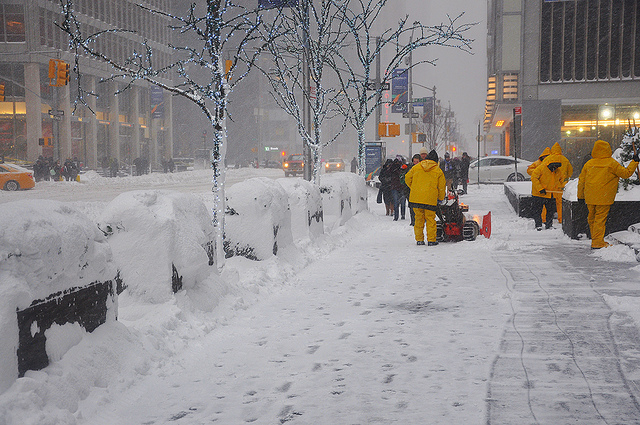
\includegraphics[width=0.12\textwidth]{image/citysnow.jpg} &
%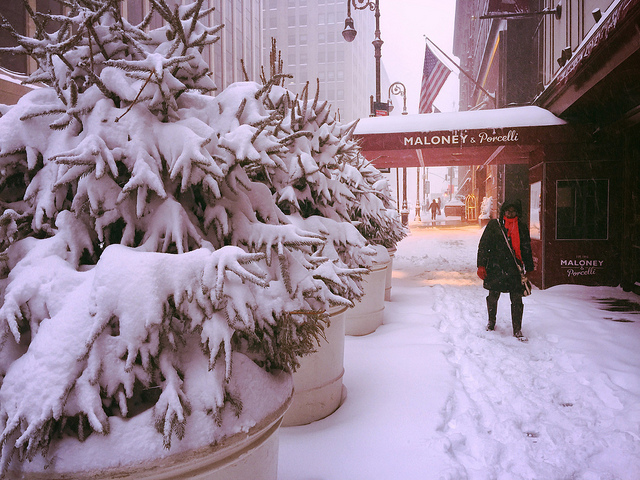
\includegraphics[width=0.1\textwidth]{image/citysnow2.jpg} &
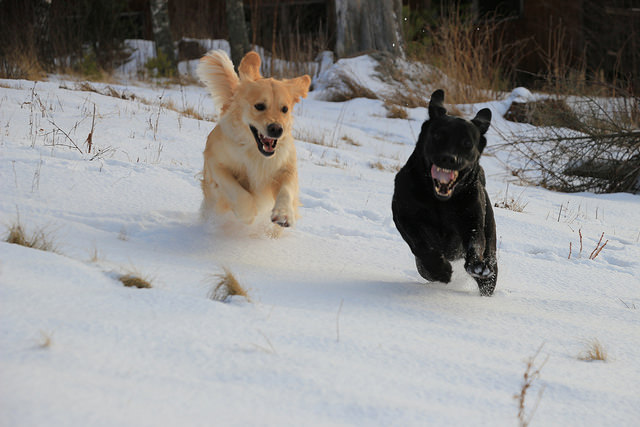
\includegraphics[width=0.15\textwidth,height=0.75in]{image/dogsnow.jpg} &
%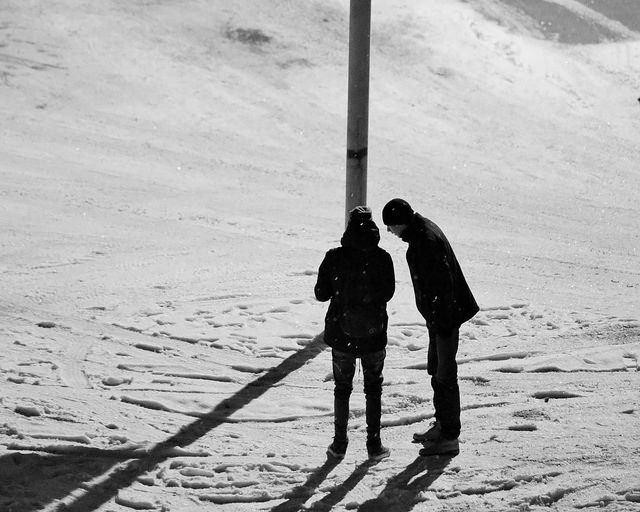
\includegraphics[width=0.1\textwidth]{image/humansnow.jpg} \\
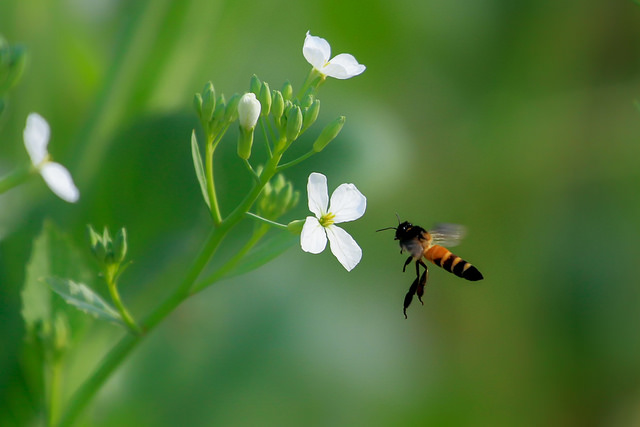
\includegraphics[width=0.15\textwidth,height=0.75in]{image/intentiongreen.jpg} &
%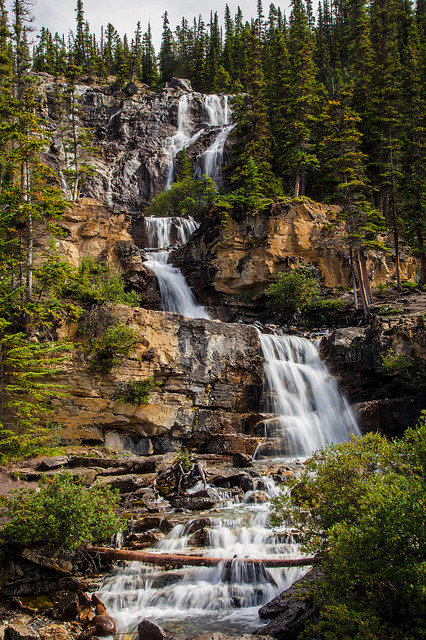
\includegraphics[width=0.1\textwidth]{image/waterfallgreen.jpg} &
%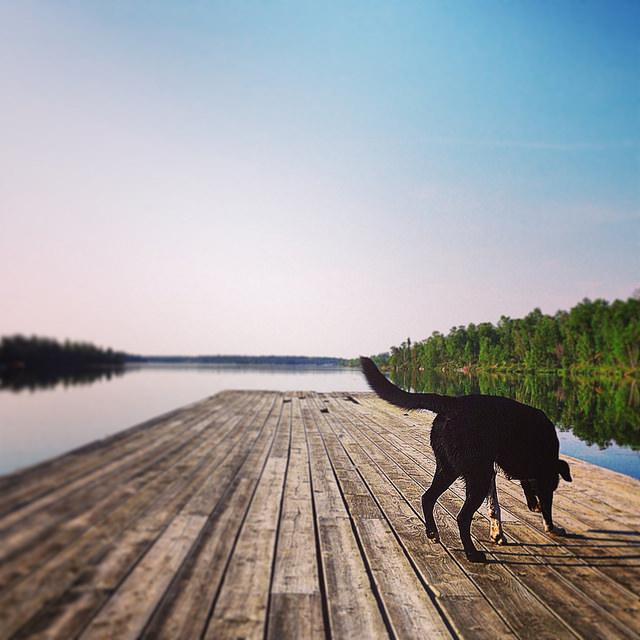
\includegraphics[width=0.12\textwidth,trim=0 0 0 cm,clip]{image/dogtree.jpg} &
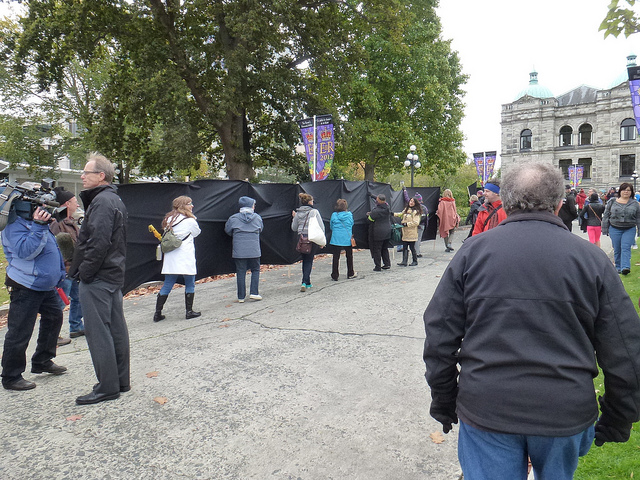
\includegraphics[width=0.15\textwidth,height=0.75in]{image/humantree.jpg} \\
\end{tabular}
\end{center}
}}
\vspace{-12pt}
\caption{Many social media images capture information about the state of the natural world, both intentionally or incidentally.}
\label{fig:flickrexp}
\vspace{-12pt}
\end{figure}


A few papers have begun to apply computer images for environmental
properties, including temperature~\cite{glasner2015hot}, cloud
cover~\cite{murdock2013webcam2satellite}, and smog conditions~\cite{li2015smog}. Most of
these papers use video data (e.g.\ from static webcams) so that visual
changes over time can be easily detected. Video camera feeds are
potentially very useful for studying longitudinal changes across time
in one particular place, but are limited to studying places where
cameras have been installed. Social photo sharing websites potentially
represent a complementary source of data, that give much greater
spatial coverage: whenever a user takes a photo at a particular place
and time and uploads it to Flickr, they are contributing a potentially
useful observation.

In this paper, we test the feasibility of leveraging these noisy and
biased images as a new source to observe nature, using modern deep
learning-based computer vision algorithms to recognize image content
automatically.  As a case study, we investigate two particular
phenomena, snowfall and vegetation coverage, since they are important
properties of the environment, they are relatively easy to recognize,
occur frequently in social images, and have satellite maps available
to serve as ground truth. This choice was also inspired by Fedorov et
al~\cite{fedorov2015snowwatch,fedorov2014snow}, who use video analysis
to monitor snow fall on mountains, and Zhang et
al~\cite{ecology2012www}, who predict snowfall from image collections
but using text tag analysis.  We first collect image data labeled to
reflect the presence of absence of ecology phenomena, and train
classifiers using Convolutional Neural Networks to recognize these
ecology phenomena in individual images. Of course, these classifiers
are noisy, and social image data is noisy also, with many inaccurate
timestamps and geo-tags.  We thus train an additional classifier that
examines all images taken at a given place and time, runs the image
classifier on each one, and then predicts if the phenomena actually
occured there and then.  Finally, we evaluate at a large scale,
training and testing on millions of Flickr images and quantiatively
evaluating the performance at hundreds of thousands of places and
times.

%% Inspried by an earlier work~\cite{ecology2012www} 
%% %\fxnote{ Fixed: cite{www}} 
%% analyzing ecology phenomenon from image tags only. We apply a new approach by 
%% understanding visual content of images, and run experiments on the exact same 
%% data set to study how vision techniques could help in social media data mining 
%% compared to using textual data alone. Also, to our best knowledge, among all the 
%% research works performing social sensing with image data, this is the first one 
%% providing continental scale quantitative performance evaluation.










\begin{figure}[t]
\centering
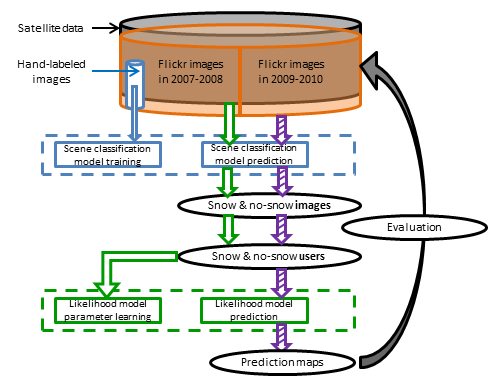
\includegraphics[scale=0.7]{figure/flowchartWevaluation.png}
\vspace{-12pt}
\caption{Overview of our approach. We train image classifiers(in blue) on large scale images. And by applying it to training images in 2007-2008, 
we train a likelihood model(in green) and finally make prediction by aggregating these visual evidence.}
% \fxnote{first classifier, then prediction}
\label{fig:overview}
\vspace{-12pt}
\end{figure}


%\input{sectionrelated}

%
% The following two commands are all you need in the
% initial runs of your .tex file to
% produce the bibliography for the citations in your paper.
\bibliographystyle{abbrv}
\bibliography{eco}  % sigproc.bib is the name of the Bibliography in this case

% You must have a proper ".bib" file
%  and remember to run:
% latex bibtex latex latex
% to resolve all references
%
\end{document}
